\section{Einführung}

\subsection{Einführung}

\begin{frame}{Chaos?}

  \begin{alertbbox}{Chaos}
    \emph{``Durcheinander, totale Unordnung''}\\[0.5ex]
    \scriptsize{\hspace{0.5ex} -- Reclam, ``Kleines Fremdwörterbuch''}
  \end{alertbbox}

  \pause

  Für unsere Zwecke:

  \begin{bbox}{Chaos bedeutet...}
    \begin{itemize}
    \item komplizierte Dynamik
    \item mit sensitiver Abhängigkeit von Anfangsbedingungen
    \end{itemize}
  \end{bbox}

  \pause

  Dennoch folgt chaotische Dynamik \alert{deterministischen} Gesetzen!
\end{frame}


\begin{frame}{Unser erstes System: das getriebene Pendel}

  \begin{columns}
    \column{0.45\textwidth}

    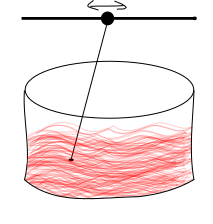
\includegraphics[width=1.05\linewidth]{Figures/Pendel.pdf}

    \column{0.55\textwidth}

    Im Ruhesystem der Aufhängung:

    \begin{itemize}
    \item rückstellende Kraft $F_1 = -mg\sin(\phi)$
    \item Kraft durch bewegte Aufhängung $F_2 = F_\mathrm{ext}$
    \item Reibung $F_3 = -2\gamma\dot{\phi}$
    \end{itemize}
    \pause
    Für harmonische treibende Kraft $F_\mathrm{ext} = A\sin(\omega_\mathrm{d}t)$:\\[-2.5ex]
    \[  m l \ddot{\phi} = -mg\sin(\phi) - 2\gamma\dot{\phi} + A\sin(\omega_\mathrm{d}t)\]
  \end{columns}
  \pause
  \vspace{1.0ex}
  Antrieb\&Dämpfung: \emph{dissipatives System}\\
  Kraft $\propto \sin(\phi)$: \alert{nichtlineares System}
\end{frame}


\begin{frame}{Pendel: kein Antrieb}

  \begin{columns}

    \column{0.5\textwidth}
    Setze $m=l=g=1$, $\gamma =0.25$, $\omega_\mathrm{d}=2/3$.\\[0.5ex]

    Zunächst $A=0$:\\[1.5ex]

    \includegraphics[width=\linewidth]{Figures/PendelA0-Zeit.pdf}

    \column{0.5\textwidth}

    \only<2,3>{

      \only<2>{DGL \emph{2. Ordnung}: Dynamik durch $\phi$ \emph{und} $\dot{\phi}$ beschrieben}

      \begin{alertbbox}{$\leadsto$ Phasenportrait}
        $\dot{\phi} = \dot{\phi}(\phi(t))$; $t$ parametrisiert die Kurve
      \end{alertbbox}
      \only<3>{
        \includegraphics[width=\linewidth]{Figures/PendelA0-Phase.pdf}}
    }

  \end{columns}

  \only<3>{$\vec\xi = (\phi, \dot{\phi}) = (0,0)$ ist ein \emph{Punkt\alert{attraktor}}}

\end{frame}


\begin{frame}{Pendel: etwas Antrieb}

  \begin{columns}

    \column{0.5\textwidth}
    Jetzt: $A=0.5$\\[1.5ex]

    \includegraphics[width=\linewidth]{Figures/PendelA05-Zeit.pdf}

    \column{0.5\textwidth}

    \only<2>{
      Phasenportrait:\\[1.5ex]
      \includegraphics[width=\linewidth]{Figures/PendelA05-Phase.pdf}
    }

  \end{columns}

  \only<2>{Die Lösungen konvergieren gegen einen \alert{Grenzzyklus} oder $1d$-Attrakor}

\end{frame}


\begin{frame}{Pendel: \emph{Mehr Power!}}

  \begin{center}
    \includegraphics[width=0.7\textwidth]{Figures/power.jpg}
  \end{center}
  \vspace{4ex}\scriptsize{Bild von http://www.mobilemag.com}
\end{frame}


\begin{frame}{Pendel: \emph{Mehr Power!}}

  \only<1,2,3>{Jetzt: $A=0$. Zwei benachbarte Anfangsbedingungen ($\omega_{\{1,2\},0}$ = 0, $\phi_{1,0} = \pi/2$, $\phi_{2,0} = \pi/2 + \delta$
    mit $\delta = 5\E{-5}$)\\[1.5ex]}

  \begin{columns}

    \column{0.5\textwidth}

    \only<2,3>{
      \includegraphics[width=\linewidth]{Figures/PendelA12-Zeit.pdf}}

    \column{0.5\textwidth}

    \only<2,3>{
      \includegraphics[width=\linewidth]{Figures/PendelA12-Phase.pdf}}

  \end{columns}

  \only<3>{Benachbarte Lösungen laufen auseinander: \alert{Chaos}!\\[0.5ex]
    $\leadsto$ Berechnung/Vorhersage schwierig/unmöglich!
  }

\end{frame}
